\sathappanc{Intro written for KDD paper}

{\em (Reference: Learning Extraction Patterns for Subjective expressions -- Ellen Riloff and Janyce Wiebe)}

Initially, a few seed phrases were obtained manually
with the help of subject matter experts. These phrases were parsed
using a dependency parser and the grammatical relationship between the
core subject word---{\em protest}, {\em manifestación}, {\em Huelga},
etc.---and any accompanying word -- {\em plan}, {\em call}, {\em anunciar} --- was extracted. To extend the initial set of phrases, a set of sentences/tweets containing a subject word and a
future time/date expression was collected and parsed.  This set of
sentences was used to expand the set of planned protest phrases by
extracting all keyword combinations that have the same grammatical
relation with respect to the core subject word. The final set of
planned protest phrases is then obtained after a manual revision of
the phrases obtained in the last step.

By this approach, we learned 122 phrases for News/blogs and 186 for tweets.


The learned phrases are then used to filter the incoming stream of Documents (news/blogs/twitter). The phrases matching is done by first splitting the incoming document into sentences and then looking for the presence of each individual word of a key-phrase (by lemma) separated by a pre-fixed maximum offset-distance (set to 3). This methodology greatly increases processing speed.

\begin{figure}
\caption{placeholder fig from an old ppt showing phrase learning}
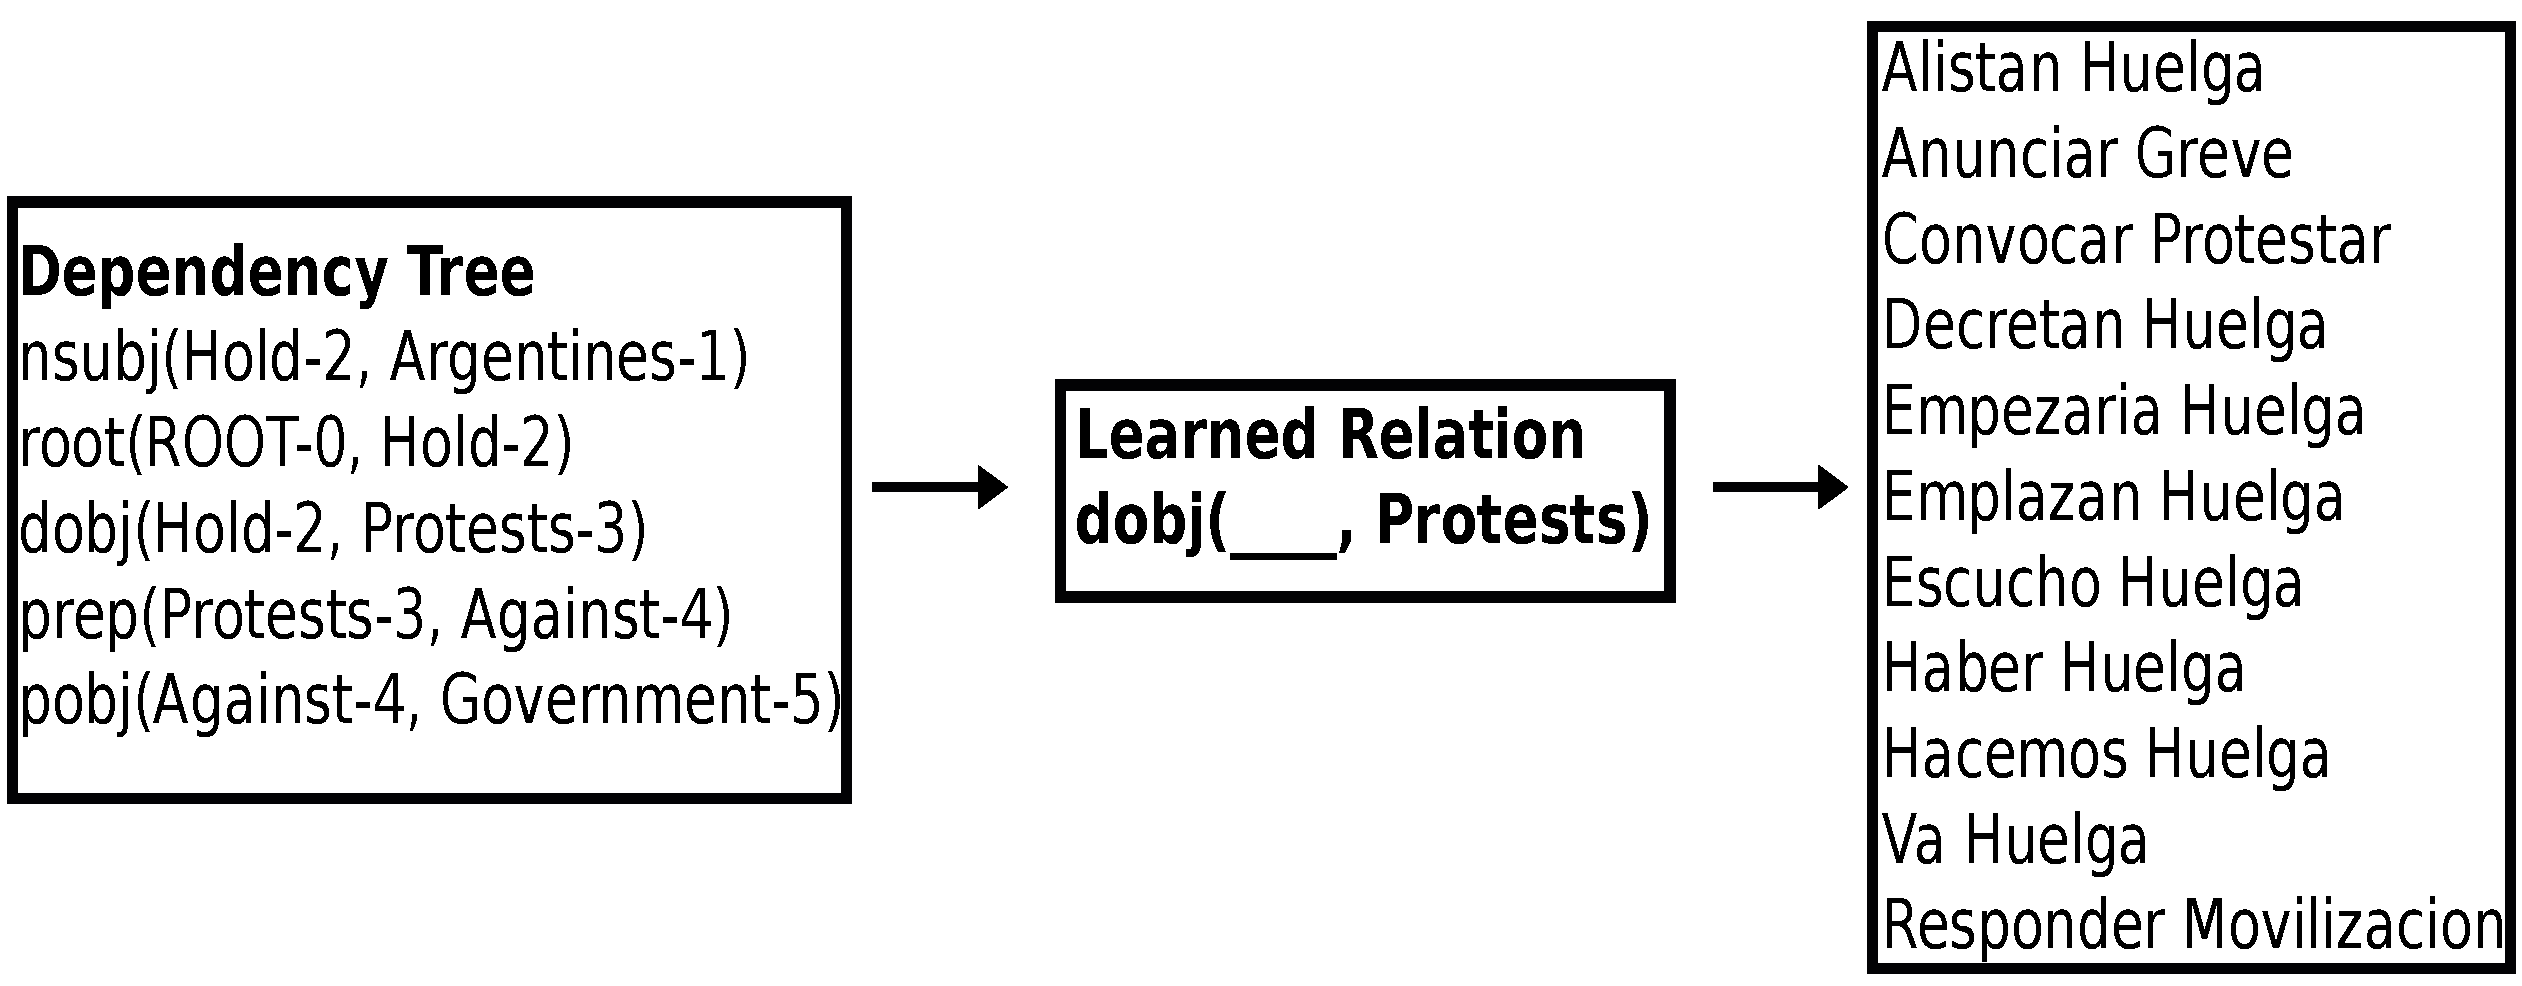
\includegraphics[width=0.5\textwidth]{figures/phraseLearning}
\end{figure}
